\documentclass[a4paper]{article}

%% Language and font encodings
\usepackage[english]{babel}
\usepackage[utf8x]{inputenc}
\usepackage[T1]{fontenc}
\usepackage{amsmath}
\usepackage{graphicx, epstopdf}
\usepackage[framed, numbered]{matlab-prettifier}
\usepackage{float}
%% Sets page size and margins
\usepackage[a4paper,top=3cm,bottom=2cm,left=3cm,right=3cm,marginparwidth=1.75cm]{geometry}

%% Useful packages
\usepackage{url}
\usepackage{amsmath}
\usepackage{graphicx,epstopdf}
\usepackage[colorinlistoftodos]{todonotes}
\usepackage[colorlinks=true, allcolors=blue]{hyperref}
\usepackage[legalpaper, landscape, margin=2in]{geometry}

\documentclass[12pt,a4paper]{article}
\usepackage{graphicx}
\usepackage{geometry}
\usepackage{background}
\geometry{a4paper,total={180mm,250mm},left=20mm,top=30mm,}
\usepackage{tikz}
\usetikzlibrary{calc}
\thispagestyle{empty}
\backgroundsetup{
scale=8,
angle=0,
firstpage=true,
opacity=0.1,
color=black,
contents={\begin{tikzpicture}[remember picture,overlay]
\node at ([yshift=1pt,xshift=0pt]current page.center)
%%{\includegraphics[width=1cm]{ceclogo.jpg}};
\end{tikzpicture}}}
\begin{document}
\begin{titlepage}

\begin{tikzpicture}[remember picture,overlay]
   \draw[line width = 2pt] ($(current page.north west) + (0.5in,-0.5in)$)  rectangle ($(current page.south east) +  (-0.5in,0.5in)$);
\end{tikzpicture}
\begin{center}
\vspace{0.8in}
\textbf{\large{DEPARTMENT OF ELECTRONIC & TELECOMMUNICATION ENGINEERING
UNIVERSITY OF MORATUWA}}\\
\vspace{0.5in}

\includegraphics[scale=0.5]{Unilogo.png}\\



\vspace{0.5in}
\textbf{EN 2570 - DIGITAL SIGNAL PROCESSING}\\
\vspace{0.5in}
\textbf{FIR Filter Design}\\
\vspace{0.5in}
\textbf{prescribed specifications using the windowing method \\in conjunction with the \\Kaiser window}\\
\vspace{1.5in}
Submitted by\\
\vspace{0.2in}
\textbf{K.R.H.M.D.M.Kularatne \hspace{8cm} 180330K}

\vspace{1cm}


\end{center}
\end{titlepage}


   





\begin{document}
\maketitle

\selectlanguage{english}
\begin{abstract}
This report is on the design of Finite Impulse Response (FIR) Bandpass Filter Using Fourier Series method along windowing method in conjunction with the Kaiser window,.Here we implement the Filter using Matlab. Here we first Implement design the filter and discuss the magnitude response of the digital filter for a frequency range. Then we add a input signal and get the Output signal with the discrete Fourier transform to demonstrate whether the correct frequencies have been passed. 
\end{abstract} \\ 
\\ 

\section{Introduction}
This report describes the sequential procedure of designing and evaluating a band pass FIR filter. The software implementation of the filter is done by MATLAB(Version R2019a, MathWorks Inc.). The filter is design by a given characteristics. Here we triging to find out the filter quality and how far its look like the idol filter. Here we use Time domain and frequency domain representation of the filter is obtained in different stages of the procedure.The frequency response of the filter was obtained primarily through the Fast Fourier Transform (FFT) implementation of Discrete Fourier Transform (DFT). Here we use a sinusoidal sum function as the input with a given and figure out where the filter is working and the difference. 

\section{Basic Theory}
A fundamental property of digital filters in general is that they have a periodic frequency response with period equal to the sampling frequency $\omega_s.$
\[ H(e^{j(\omega +k\omega_s)T} = H(e^{j(\omega T))})\]
Since the frequency response is periodic we can represent it as a Fourier Series as below.
\[H(e^{j(\omega T))} =  \sum_{-\infty}^{\infty} h(nT)e^{-j(\omega nT))} \]
where,
\[h(nT) = \frac{1}{\omega_s}\int_{\omega_s / 2}^{-\omega_s / 2} H(e^{j(\omega T))}e^{-j(\omega nT))} \,dx \ \]
    
Define the impulse response of the Filter as $h(nT)$and then by By substituting $ z = e^{j(\omega T))} $ we obtain the Transfer function of the filter as follows.
\[H(z) =  \sum_{-\infty}^{\infty} h(nT)z^{-n} \]

Since the Fourier series coefficients are defined over the range $-\infty < n <\infty$ there are two problems regarding the Fourier series method.
\begin{itemize}
  \item The nonrecursive filter obtained is of infinite length.
  \item The filter is noncausal because the impulse response is nonzero for negative time.
\end{itemize}
A finite filter length can be achieved by truncating the impulse response in such way that,
h(nT ) = 0 for |n| > M where M = (N - 1)/2. And a causal filter can be obtained by delaying the impulse response by a period MT seconds or by M sampling periods.
Since delaying the impulse response by M sampling periods amounts to multiplying the transfer function by $z^{-M}$, the transfer function of the causal filter has the following form.
\[H'(z) = z^{-M} \sum_{-\infty}^{\infty} h(nT)z^{-n} \]

and we obtain the frequency response as,
\[H'(e^{j(\omega T)}) = e^{-jM(\omega T)} \sum_{-\infty}^{\infty} h(nT)e^{-jn \omega T} \]

The amplitude response of the filter does not change with the sample shift as $|e^{-jn \omega T}| = 1 $.
However, the phase response will change from that of the original.

However, we can observe that the amplitude response of the filter would have undesirable oscillations (Gibbs oscillations) in both the stop band and the pass band. They are caused by the truncation of the Fourier series. And unfortunately we cannot reduce this phenomenon by increasing the truncation length.

As a solution this problem we use a window function $ W(nT )$ to truncate the infinite duration filter response $h(nT )$. This is done as follows.
\[h_w(nT ) = h(nT)W(nT) \]
So the Transfer function of the modified filter is,
\[H_w(nT ) = Z[h(nT)W(nT)] \]

Therefore the frequency response of the modified filter is ,
\[H_w(e^{j(\omega T))} =  \frac{T}{2\pi}\int_{2\pi /T}^{0} H(e^{j\omega' T})W(e^{j(\omega -\omega')T))} \,d\omega' \ \]

%figure

Windows are characterized by their main-lobe width, $A_{ML}$, which is the bandwidth between the first negative and the first positive zero crossings, and Maximum side-lobe $A_{max}$ by their ripple ratio, R, which is defined as,
\[R = 20\log(\frac{A_{max}}{A_{ML}})\]

The main-lobe width and ripple ratio should be as low as possible. The spectral energy of the window should be concentrated as far as possible in the main lobe and the energy in the side lobes should be as low as possible. Though there are many window functions available here we use Kaiser Window to implement the filter.

\section{Kaiser Window}
The Kasier window function is given by,
\[
     w_K(nT) = \begin{cases}
     \tfrac{I_0(\beta)}{I_0(\alpha)} & for \hspace*{3pt} \abs{x}  \leq \frac{N-1}{2} \\
     0 & otherwise
    \end{cases}
    \]\\
where $\alpha$ is an independent parameter,\\
    \[\beta = \alpha\sqrt{1-\left(\frac{2n}{N-1}\right)^2} \]
    and
    \[I_0(\alpha) = 1+\sum_{k=1}^{\infty}\left[\frac{1}{k!}\left(\frac{x}{2}\right)^k\right]^2\]
Here $I_0(x)$ is a zeroth-order modified Bessel function of the first kind.
% figure2
% figure3
A filter-design method is available, also proposed by Kaiser, that can be used to design nonrecursive filters that would satisfy arbitrary prescribed specifications. This method can be
used to design lowpass (LP), highpass (HP), bandpass (BP), and bandstop (BS) filters. Here we tring to implement a bandpass filter.

\\



\section{Design}
The design specification are as follows,
    \begin{center}
    \begin{table*}[h]
    \centering
    \caption {Required Filter Specifications}
     This table provides the required bandstop characteristics of the digital filter\\
    \begin{tabular}{@{}lccl@{}}
        \toprule
            {Specification} & {Symbol} & {Value} & {Units}  \\
            \midrule
            Maximum pass band ripple & $\tilde A_p$         & 0.06  & dB  \\
            Maximum stop band attenuation & $\tilde A_a$    & 48    & dB  \\
            Lower pass band egde & $\Omega_{p1}$            & 300   & rad$s^{-1}$  \\
            Upper pass band edge & $\Omega_{p2}$            & 700  & rad$s^{-1}$  \\
            Lower stop band egde & $\Omega_{a1}$            & 150  & rad$s^{-1}$  \\
            Upper stop band edge & $\Omega_{a2}$            & 800  & rad$s^{-1}$  \\
            Sampling frequency & $\Omega_s$                 & 1200  & rad$s^{-1}$  \\
        \bottomrule
    \end{tabular}
    \end{table*}
    \end{center}
    \vspace*{-25pt}
    
\begin{figure}[h]
    \centering
    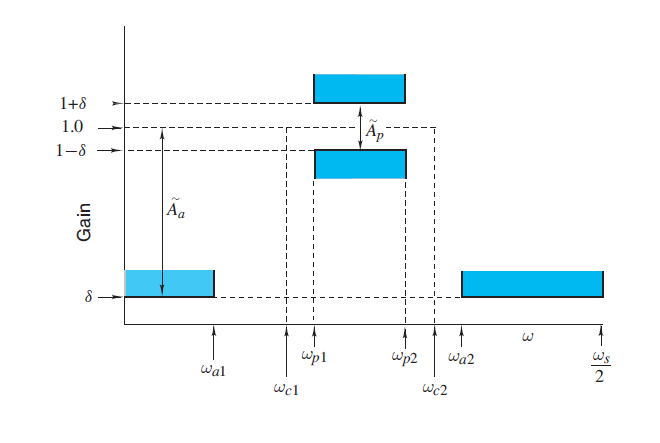
\includegraphics[width=1\textwidth]{bandpass figure.png}
    \caption{Filter Specification}
    \label{fig:mesh1}
\end{figure}


\begin{center}
\begin{table*}[h]
\centering
\caption {Derived Filter Specifications}

This table provides the derived bandstop characteristics of the digital filter 
\begin{tabular}{@{}lcccl@{}}
    \toprule
        {Specification} & {Symbol} & {Derivation} & {Value} & {Units}  \\
        \midrule
        Lower transition width & $B_{t1}$           & $\omega_{a1}-\omega_{p1}$   & 150     & rad$s^{-1}$  \\
        Upper transition width & $B_{t2}$           & $\omega_{p2}-\omega_{a2}$   & 100     & rad$s^{-1}$  \\
        Critical transition width & $B_t$           & $min[B_{t1},B_{t1}]$        & 100     & rad$s^{-1}$  \\
        Lower cutoff frequency & $\omega_{c1}$      & $\omega_{p1}+\frac{B_t}{2}$ & 250     & rad$s^{-1}$  \\
        Upper cutoff frequency & $\omega_{c2}$      & $\omega_{p2}-\frac{B_t}{2}$ & 750    & rad$s^{-1}$  \\
        Sampling period & $T$                       & $\frac{2\pi}{\omega_s}$     & 0.0026  & s  \\
    \bottomrule
\end{tabular}
\end{table*}
\end{center}
From the above specifications, the more critical transition width is,
\[B_t = min[(\Omega_{a1}-\Omega_{p1}),(& \Omega_{p2}-\Omega_{a2})]\]

Hence, idealized frequency response for a Bandpass filter is given as,
\[H(e^{i\omega T}) = \begin{cases}
     0 & for \hspace{0.2cm} 0 \leq |\omega| \leq \omega_{c1} \\
     1 & for \hspace{0.2cm} \omega_{c1} \leq |\omega| \leq \omega_{c2} \\
     0 & for \hspace{0.2cm} \omega_{c2} \leq |\omega| \leq \omega_{s}/2 
    \end{cases}
    \]
    
Appling the Fourier series to the idealized frequency response , we get
\[h(nT) = \begin{cases}
     \frac{2}{\omega_s} & for \hspace{0.2cm} n=0 \\
     \frac{1}{n\pi}(\sin{\omega_{c2}nT }-\sin{\omega_{c1}nT ) &  Otherwise 
    \end{cases}
    \]
Now we applying the theories for the design
\begin{enumerate}
  \item Choose a suitable values for $\delta$ using the below equations.
  $$\tilde{\delta_p}=\frac{10^{0.05\tilde{A_p}}-1}{10^{0.05\tilde{A_p}}+1} \hspace*{25pt}and\hspace*{25pt} \tilde{\delta_a}=10^{-0.05\tilde{A_a}}$$
  
 which,
 $\delta = min(\tilde{\delta_p},\tilde{\delta_a})$
  \item Calculate the actual stop band attenuation $A_a$ by.
  $$A_a = -20log\abs{x}$$
  \item Choose parameter $\alpha$ as,
  $$\alpha = \begin{cases}
     0 & for \hspace{0.2cm} A_a \leq 21 \\
     0.5842(A_a-21)^0.4 + 0.07886(A_a-21)  & for \hspace{0.2cm} 21 < A_a l \leq 50 \\
     0.1102(A_a-8.7) & for \hspace{0.2cm} A_a  > 50
    \end{cases}
$$
    \item Choose parameter D as,
    \[
     D = \begin{cases}
     0.9222 & for \hspace*{3pt} A_a \leq 21 dB \\
     \frac{A_a - 7.95}{14.36} & for \hspace*{3pt} A_a > 21 dB
    \end{cases}
    \]
    
    \item Select the lowest odd value of N that would satisfy the inequality,
    $$N\geq\frac{\omega_sD}{B_t}+1$$\\
    \item Now we can use the Kaiser Window Method which describe in the Theory part
\end{enumerate}
\pagebreak
\section{Results}
The Following design specifications were used in the project,
%table
the Results are as follows,
The results of the filter design can be presented in two forms. The characteristics of the filter in each stage of the filter design process can be seen by the impulse response and frequency response plots. The performance of the filter can be evaluated by comparing the input and output obtained by the filter evaluation stage. Here we use Matlab for plot the graphs and 

\subsection{Frequency and Time Domain plots of the Filter}
The following plots were obtained during the procedure of designing the filter. Impulse response of the Kaiser Window is shown in figure 2. Frequency response of the filter when a Rectangular Window was used is shown in figure 3. Impulse response of the filter when a Rectangular Window was used is shown in figure 4. Frequency response of the filter when a Kaiser Window was used is shown in figure 5. Impulse response of the filter when a Kaiser Window was used is shown in figure 6. A zoomed in plot of the pass band of the signal is obtained in order to visually identify the pass band ripples, as shown in figure 7.
\begin{figure}[H]
    \centering
    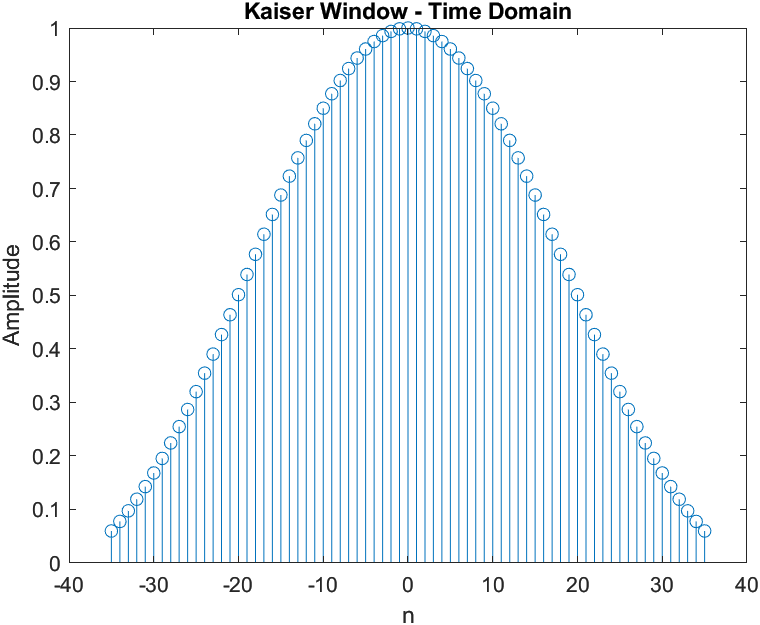
\includegraphics[width=0.8\textwidth]{untitled1.png}
    \caption{}
    \label{fig:mesh1}
\end{figure}

\begin{figure}[H]
    \centering
    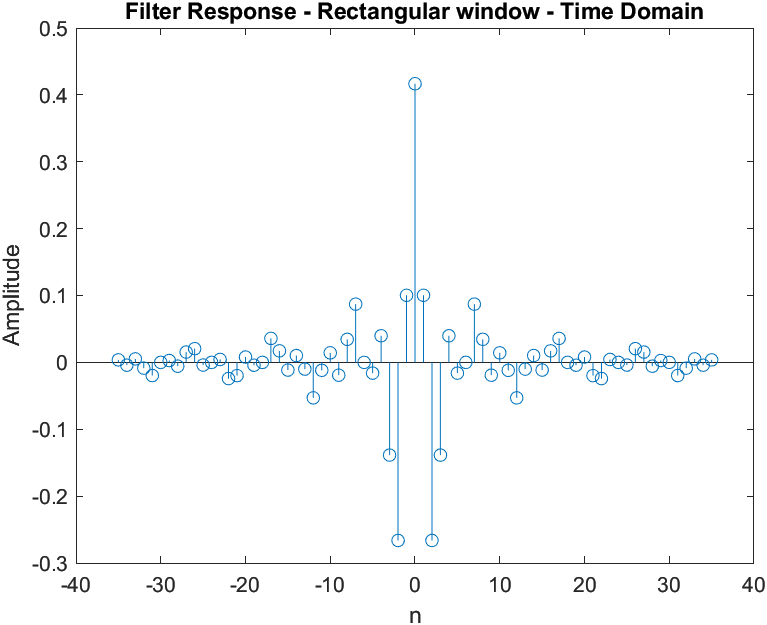
\includegraphics[width=0.8\textwidth]{untitled2.png}
    \caption{}
    \label{fig:mesh1}
\end{figure}

\begin{figure}[H]
    \centering
    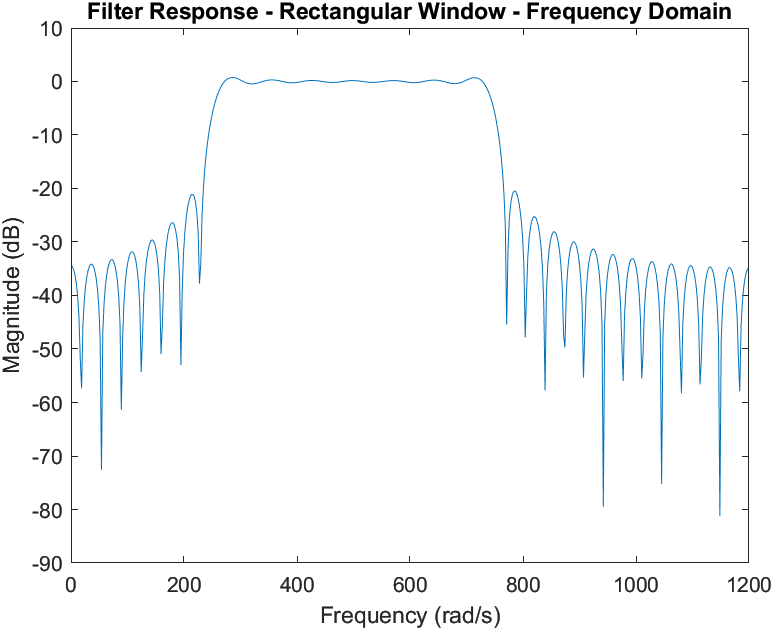
\includegraphics[width=0.8\textwidth]{untitled3.png}
    \caption{}
    \label{fig:mesh1}
\end{figure}

\begin{figure}[H]
    \centering
    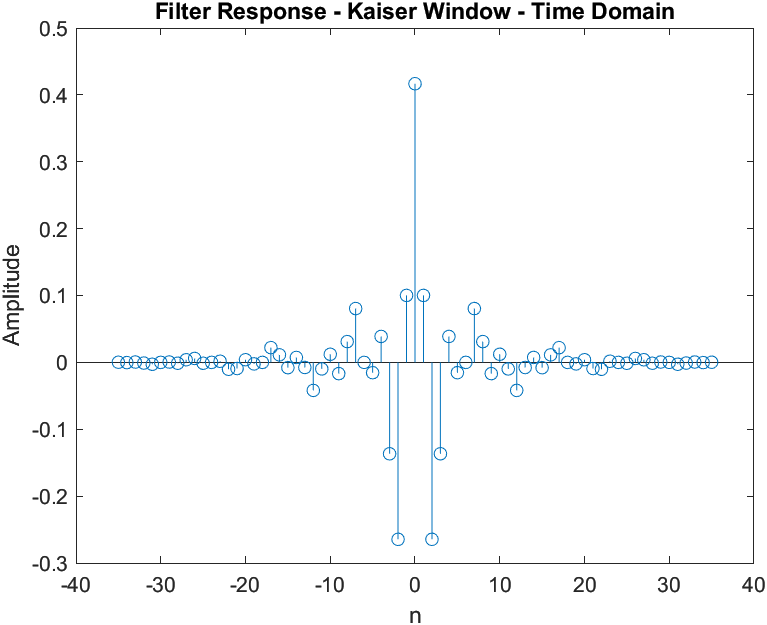
\includegraphics[width=0.8\textwidth]{untitled4.png}
    \caption{}
    \label{fig:mesh1}
\end{figure}

\begin{figure}[H]
    \centering
    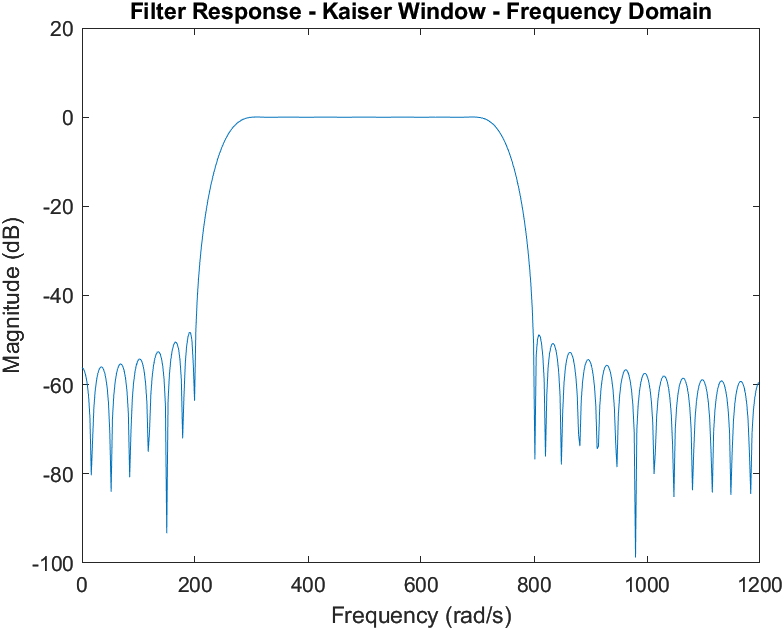
\includegraphics[width=0.8\textwidth]{untitled5.png}
    \caption{}
    \label{fig:mesh1}
\end{figure}

\begin{figure}[H]
    \centering
    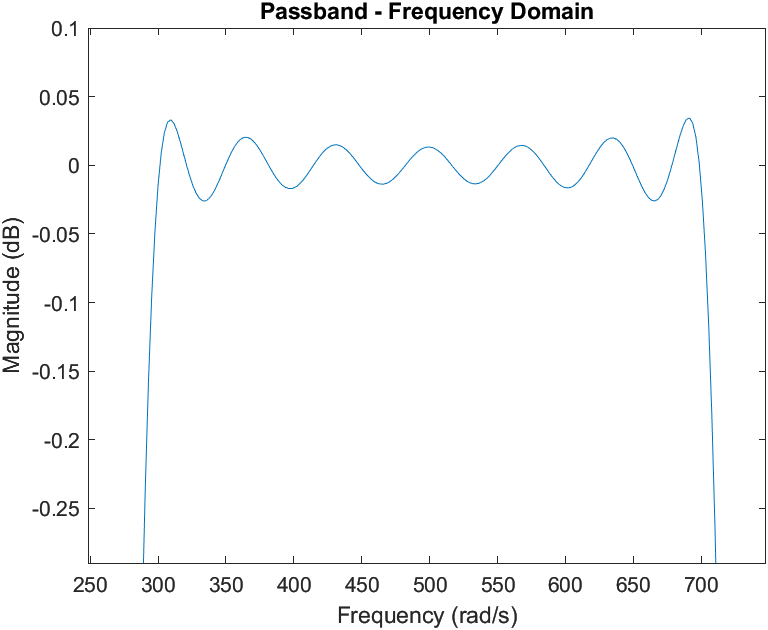
\includegraphics[width=0.8\textwidth]{untitled6.png}
    \caption{}
    \label{fig:mesh1}
\end{figure}
\pagebreak

\subsection{Validation of the designed bandpass filter}
For the validation purposes, the following time domain excitation was used.
\[ x(nT) =\sum_{i=1}^{3} \sin{(\omega_i nT) }\]
Since the cutoff frequencies of the designed bandpass filter was $\Omega_{c1} = 250 rads^{-1} and \Omega_{c2} = 750 rads^{-1}  $.
so the relevant values for 
\[\Omega_1 = 125 rads^{-1}\]
\[\Omega_2 = 500 rads^{-1}\]
\[\Omega_3 = 975 rads^{-1}\]
was chosen as the frequencies of the excitation signal.
As it was observed, the filtered signal using the bandpass filter and the ideally filtered signal were almost the same.
\vspace{3cm}
\begin{figure}[H]
    \centering
    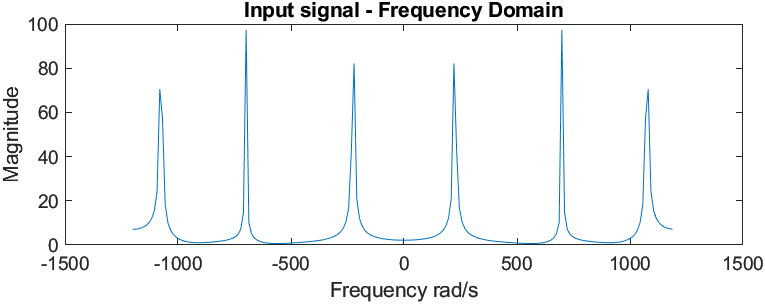
\includegraphics[width=0.7\textwidth]{untitled7.png}
    \label{fig:mesh1}
\end{figure}

\begin{figure}[H]
    \centering
    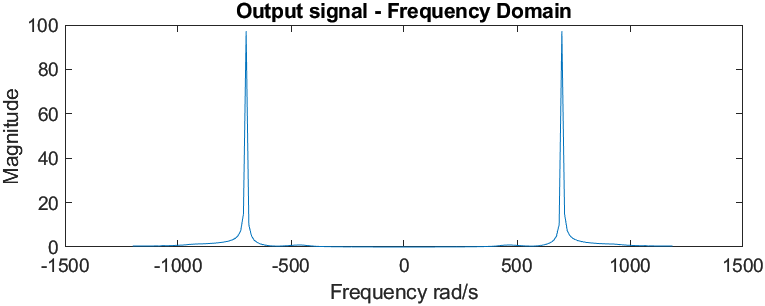
\includegraphics[width=0.7\textwidth]{untitled8.png}
    \label{fig:mesh1}
\end{figure}
\vspace{5cm}
\begin{figure}[H]
    \centering
    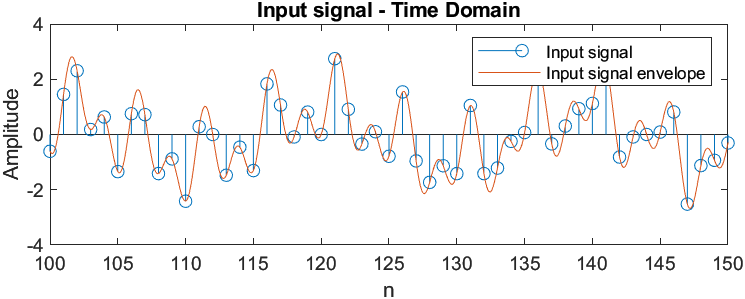
\includegraphics[width=1\textwidth]{untitled11.png}
    \caption{Input signal - Time Domain}
    \label{fig:mesh1}
\end{figure}

\begin{figure}[H]
    \centering
    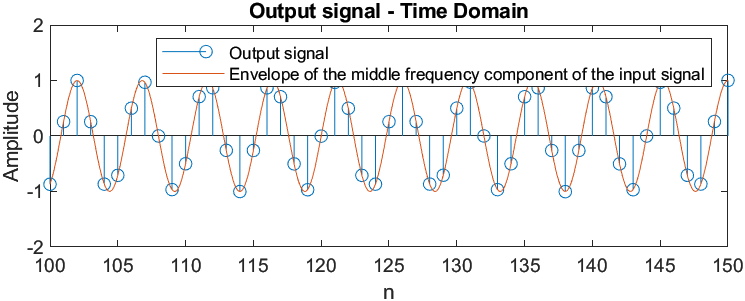
\includegraphics[width=1\textwidth]{untitled12.png}
    \caption{Output signal - Time Domain}
    \label{fig:mesh1}
\end{figure}
\pagebreak
\section{Discussion}
There several significant differences between the filter obtained by Rectangular Window and the Kaiser Window.Here we can see some advantages well as the disadvantages in this window method. As we consider the FIR designs with window will use Finite response and have trying to be more idol filter. Here with the Kaiser window we can see main three features.Less stopband attenuation,kaiser window has less ripple,passband edge distortion less as the advantages. Here we can see Kaiser window is more complex than the rectangular window so as i think the implementation part will be much harder.

\section{Conclusion}
We can use Kaiser window instead of rectangular window for more realistic idol filter. Though it has some ripples and stopband attenuation it is more likely the idol one instead of rectangular window. But Implementation is more Complex .

\section{Acknowledgement}
I would like to express our gratitude to Dr. Chameera Edirisooriya, the project supervisor, for the constant guidance he provided throughout this project.Also I thank my colleagues for sharing their knowledge and experience on this project.

\begin{thebibliography}{9}
\bibitem{a_reference} A. Antoniou, "Digital Signal Processing," 2005. [Online]. Available: www.ece.uvic.ca/~dsp. [Accessed 29 12 2016].

\bibitem{b_reference}https://en.wikipedia.org/wiki/$Kaiserwindow$.

\bibitem{other_ref} Digital Signal Processing: Signals, Systems, and Filters 1st Edition by Andreas Antoniou


\end{thebibliography}
\pagebreak
\lstinputlisting[style=Matlab-editor , caption={Matlab Code.}]{bandPass.m}
\end{document}\end{document}